Niniejszy rozdział opisuje zakres działań podjętych w celu stworzenia aplikacji
sterujących robotem Dark Explorer (rys. \ref{fig:DarkExplorerPlatformStacMob}). Przedstawiony jest
zestaw narzędzi niezbędnych do rozwoju oprogramowania dedykowanego dla robota na urządzenia mobilne oraz
komputery stacjonarne. Opisano także możliwości stworzonych aplikacji, sposób
instalacji i~użytkowania.

\begin{figure}[!ht]
 \centering
 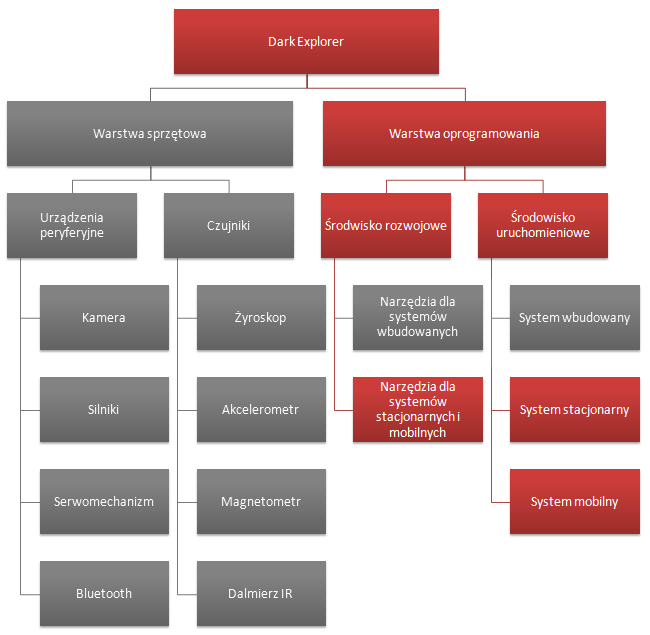
\includegraphics[height=125mm]{../images/ch03/dark_explorer_platform_ide_stac_mob.png}
 \caption{Struktura platformy robota mobilnego po zakończeniu prac. Kolorem
 niebieskim oznaczono zakres prac opisanych w bieżącym rozdziale.}
 \label{fig:DarkExplorerPlatformStacMob}
\end{figure}

\section{Biblioteki programistyczne do zarządzania robotem}
Jednym z poważniejszych problemów zauważonych podczas analizy pierwotnej
konfiguracji robota był brak bibliotek umożliwiających tworzenie oprogramowania,
które pozwalałoby na dowolne wykorzystanie możliwości oferowanych przez
konfigurację sprzętową robota. Brak tego rodzaju narzędzi znacząco ogranicza
możliwości rozwoju robota, gdyż każda próba tworzenia nowego oprogramowania wymaga
od programisty zagłębiania się w szczegóły implementacji systemu wbudowanego,
który kontroluje działanie robota. Aby usunąć tak poważne ograniczenie,
zaprojektowana została biblioteka mająca na celu udostępnienie narzędzi,
pozwalających programiście na skupienie się jedynie na wysokopoziomowej
funkcjonalności, bez konieczności szczegółowej analizy protokołu komunikacji i
zasad działania poszczególnych funkcji robota.

Przed przystąpieniem do implementacji konieczne jest podjęcie rozważnej decyzji z
wyborem środowiska i języka programowania w jakim biblioteka zostanie napisana.
Biorąc pod uwagę ciągle rosnącą popularność obiektowych języków programowania
oczywistym wydaje się być wybór języka właśnie z tej rodziny. Decydującym
aspektem, wpływającym na ostateczny wybór docelowej platformy rozwojowej, jest
więc ilość dostępnych bibliotek oraz przenośność kodu pomiędzy dostępnymi na
rynku platformami sprzętowymi. Po przeprowadzeniu wnikliwej analizy ostateczny
wybór padł na dwa rozwiązania: język C\# z platformą .NET oraz język Java. 
Wybór motywowany jest faktem iż platforma .NET jest jednym z najdynamiczniej rozwijających środowisk
programistycznych ostatnich lat natomiast Java jest niesamowicie popularna i dostępna w obecnych środowiskach uruchomieniowych. 

\subsection{Platforma .NET}
\label{subsec:sdk-.net}
Firma Microsoft dostarcza szereg bibliotek dodatkowych oraz narzędzi pozwalających na szybkie tworzenie oprogramowania
działającego zarówno na urządzeniach mobilnych jaki i stacjonarnych. Dzięki
pracy programistów w ramach projektu Mono\footnote{Więcej informacji na temat projektu
Mono można znaleźć pod adresem strony internetowej http://www.mono-project.com/}
powstała platforma umożliwiająca uruchamianie aplikacji napisanych w języku C\#
nie tylko pod kontrolą systemu Windows, ale również pod systemami z rodziny Linux
i Mac. Dodatkowym atutem platformy .NET jest bardzo duża liczba bibliotek
dodatkowych dostarczanych przez środowiska programistów opensource.

W ramach pracy magisterskiej zaprojektowana została biblioteka programistyczna w
języku C\#. Docelową platformą uruchomieniową dla przygotowanej biblioteki są
systemy z rodziny Windows, Windows Mobile oraz Linux. Przy tworzeniu biblioteki
brane pod uwagę były najnowsze trendy w dziedzinie programistycznych wzorców
projektowych przy jednoczesnym zachowaniu spójności i uniwersalności kodu dla
poszczególnych środowisk uruchomieniowych. W wyniku implementacji powstała
wielowątkowa biblioteka oparta na zdarzeniach pozwalająca na dostęp do wszystkich
funkcji robota za pomocą intuicyjnego interfejsu programistycznego. Biblioteka
udostępnia szerokie spektrum metod pozwalających na swobodne sterowanie i
zarządzanie dostępnymi funkcjami robota. Wśród metod bibliotecznych znaleźć można
funkcje pozwalające na bezpośrednią interakcję z poszczególnymi podzespołami
bazowymi, jak również takie które umożliwiają wykonywanie predefiniowanych
sekwencji zadań przewidzianych przez autorów projektu. Biblioteka pokrywa swoją
funkcjonalnością nie tylko wsparcie dla wszystkich dostępnych rozszerzeń
sprzętowych robota, ale również dostarcza interfejs pozwalający na automatyczną
obsługę połączenia z robotem z wykorzystaniem technologii bluetooth. Fakt ten
jest o tyle istotny, że proces komunikacji okazał się być najbardziej wrażliwym
elementem podczas migracji biblioteki pomiędzy poszczególnymi platformami
softwareowymi. Szczegółowa lista wszystkich dostępnych funkcji wraz z niezbędnym
komentarzem, zamieszczona została w dodatku poświęconym kodowi źródłowemu,
stworzonemu w ramach pracy magisterskiej. Taki sposób implementacji pozwala na
tworzenie oprogramowania współpracującego z nową wersją robota nawet przez osoby
nie posiadające dostatecznej wiedzy i umiejętności tworzenia oprogramowania do
obsługi systemów wbudowanych.

W ramach pracy magisterskiej stworzona została również przykładowa aplikacja
sterująca prezentująca wszystkie możliwości oferowane zarówno przez warstwę
aplikacyjną jak i sprzętową robota Dark Explorer. Do wykonania aplikacji
klienckiej wykorzystana została omawiana powyżej biblioteka programistyczna.
Stanowi ona przewodnik dla początkującego programisty pokazujący w jaki sposób
można wykorzystać udostępnione funkcje biblioteczne. Okno główne aplikacji
widoczne jest na rysunku \ref{fig:win-ctrl-app}. Program umożliwia
sterowanie zarówno manualne jak i sterowanie półautomatyczne
po włączeniu trybu rekonstrukcji ścieżki czy rozpoznawania obrazu. Korzystając z
menu głównego aplikacji użytkownik może dokonywać kalibracji czujników i
przeprowadzać za ich pomocą dowolne pomiary. Dodatkowo w aplikacji udostępniona
została historia wykonywanych akcji. Jest to bardzo przydatne narzędzie
pozwalające na bieżąco śledzić nie tylko stan aplikacji ale~również robota. Dla
wygody użytkownika większość dostępnych funkcji została zgrupowana w
menu głównym aplikacji. Dzięki takiemu podejściu użytkownik może bardzo szybko
uzyskać dostęp do interesującej go funkcji bez konieczności przedzierania się
przez dużą ilość kontrolek w oknie głównym aplikacji. 
\newpage

\begin{figure}[!ht]
 \centering
 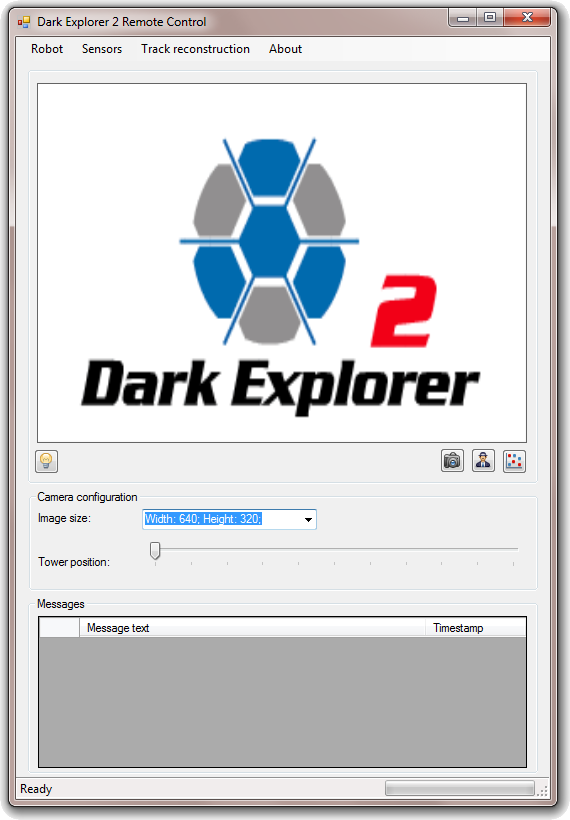
\includegraphics[height=150mm]{../images/ch05/win-ctrl-app.png}
 \caption{Okno główne aplikacji sterującej napisanej w języku C\#}
 \label{fig:win-ctrl-app}
\end{figure}

\newpage

\subsection{Biblioteka zarządzająca dla języka Java}
\label{subsec:sdk-java}
Drugim rozwiązaniem programistycznym umożliwiającym sterowanie robotem za pomocą
urządzeń zewnętrznych jest biblioteka napisana w języku Java. Pozwala ona na
komunikowanie się z robotem przy pomocy prostych funkcji, które nie wymagają od
programisty żadnej wiedzy na temat mechanizmów przesyłu danych pomiędzy robotem a
resztą świata. Podobnie jak w przypadku biblioteki przygotowanej pod platformę
.NET możemy bezpośrednio sterować poszczególnymi podzespołami bazowymi wysyłając
własne komendy lub też korzystać z funkcji wbudowanych, odpowiedzialnych za
wykonywanie konkretnych czynności, np.: manewrowanie robotem, pobieranie zdjęcia
w określonej rozdzielczości, kontrolowanie serwomechanizmu.

Biblioteka została podzielona na dwie klasy. Jedna z nich jest odpowiedzialna za
obsługę komunikacji bluetooth pomiędzy aplikacją a robotem Dark Explorer. Druga
natomiast pozwala w łatwy sposób wykorzystywać wszystkie funkcje robota.

Biblioteka była tworzona docelowo na telefony komórkowe z wbudowaną maszyną
wirtualną Java, które implementują API do komunikacji bluetooth JSR
82\footnote{JSR 82 - Java Specification Request, zbiór reguł których należy się
trzymać podczas implementacji API do komunikacji bluetooth}. Możliwe jest również
wykorzystanie tej biblioteki na komputerach stacjonarnych. W tym celu konieczne
jest wyposażenie tworzonej aplikacji w bibliotekę wspierającą JSR 82. Dostępnych
jest kilka tego rodzaju bibliotek (tab. \ref{tab:JSR82SDK}).

\begin{table}[hb]
  \rowcolors{2}{white}{gray!20}
  \centering
  \caption{Biblioteki wspierające JSR-82\cite{website:javabluetooth.com}}
  \begin{tabular}{ | c | c | c | c | c | c |} \hline
    Nazwa & Wsparcie & Wsparcie & Platformy & Obsługiwane & Cena \\
    & bluetooth\footnotemark & OBEX\footnotemark & Java & systemy & \\ \hline Avetana & Tak & Tak &
    J2SE & Win-32, Mac OS X & 25\euro \\ & & & & Linux, Pocket PC & \\ \hline BlueCove & Tak & Tak & J2SE & Win-32, Mac OS X & darmowa \\ \hline
    Electric Blue & Tak & Tak & J2SE & Win XP SP2 & 15\$ \\ \hline
    Harald & Nie & Nie & każda z  & wiele & darmowa \\
    & & & javax.comm  &  & \\ \hline
    JavaBluetooth.org & Tak & Nie & każda z  & wiele & darmowa \\
    & & & javax.comm  &  & \\ \hline
    Rococo & Tak & Tak & J2SE J2ME & Linux, Palm OS & 2500\euro \\ \hline
  \end{tabular}
  \label{tab:JSR82SDK}
\end{table} 

\footnotetext[3]{Mowa tutaj o klasach i interfejsach dostępnych w
    ramach pakietu javax.bluetooth zgodnych z wymaganiami JSR 82}
\footnotetext[4]{Mowa tutaj o klasach i interfejsach dostępnych w
    ramach pakietu javax.obex zgodnych z wymaganiami JSR 82}